\chapter{Evaluation}
\label{chap:evaluation}

This chapter intent is to describe the evaluations preformed against the solution. For that the following sections will tackle:

\begin{itemize}
    \item Objectives and execution environment of this evaluation;
    \item Approach applied to evaluate the software developed;
    \item Drafted experiences and results collected;
    \item Analysis of the results collected;
    \item Observations taken from the analysis conducted.
\end{itemize}

The expected behavior of the system according to functional requirements can be attested with deterministic tests presented in Section~\ref{sec:implementation:testing}. On the other hand, some non-functional requirements, such as performance and usability requirements, can't be deterministically attested with simple tests.

Since the company and this project's solution were both in the early stages of conception no strick usability requirements were defined. The experiences here documented focus on the performance of the solution according to the points defined in Section~\ref{sec:requirements:non_functional}.

\section{Objectives}
\label{sec:evaluation:objectives}

The objective of this evaluation is to determine the throughput limits of the entire solution (\textbf{Sensae Console} and \textbf{External Services}) regarding data ingestion, within the requirements detailed in Section~\ref{sec:requirements:non_functional}.

Since the solution was designed to scale infinitely and handle high-levels of throughput, the performance of it in a multi-organization and shared infrastructure is undermined. The evaluation should instead focus on environments where resources are constrained.

Therefore, the performance of the solution will be tested against above-average usage conditions of small to medium organizations that require a dedicated infrastructure, either on-site or in the cloud.

This type of organizations encompass entities such as:

\begin{itemize}
    \item Public Institutes: town councils, public transportation organizations, waste management departments and others;
    \item Private owned business: chicken farms, greenhouse farms, goods transportation agencies, industrial warehouses, agriculture cooperatives and others;
\end{itemize}

The objective is to determine the platform limits of data ingestion, processing, storage and real-time supply within the desired requirements.

This evaluation also helps to understand what components are the first to degrade the performance of the system.

\section{Approach}
\label{sec:evaluation:approach}

The approach taken to evaluate the solution was to send increasingly higher volumes of HTTP requests to the \nameref{subsec:implementation:description:ingestion} in order to determine the platform limits of healthy operation.

Given the type of organizations that require this deployment mode it is expected that the number of devices installed doesn't go beyond 500\footnote{500 devices in use by a single entity is expected to be a huge amount of devices for the realistic business needs of small/medium organizations}.

The evaluation encompasses 4 test scenarios, one for the developed platform and one for each developed service: (i) Sensae Console, (ii) Fleet Management, (iii) Smart Irrigation, (iv) Notification Management.

The performance tests use the \citetitle{k6} tool. This tool allows one to design performance tests entirely in \textit{Javascript}. An example of the scripts developed is presented in Appendix~\ref{AppendixF}. The \citetitle{k6} tool produces various metrics that are then analyzed using \textit{R}, an example of the analysis scripts developed is presented in Appendix~\ref{AppendixG}.

For simplicity, the solution was deployed in a \gls{VM} Instance of the Google Cloud Platform, type \textit{'e2-standard-4'}, with the following specs:

\begin{itemize}
    \item Memory: 16 GB;
    \item Number of vCPU Cores: 4;
    \item Disk Type: Balanced Persistence Disk.
\end{itemize}

As of September, 2022, the cost associated with this \gls{VM} rounds the 100\texteuro per month.

These tests were executed through the author' machine which may undermine the communication with the \gls{VM} Instance, e.g. number of HTTP requests and stability of the Websocket connection.

The approach taken isn't an attempt to mimic normal usage patterns but simply to envision the platform throughput limits. Even though an approach closer to the reality would present results easier to interpreter, it would take to much time to design, implement and run these realistic tests. Therefore, metrics such as the interval between two consecutive Uplinks of the same device, were severely narrowed.

\section{Experiences}
\label{sec:evaluation:experiences}

As described before, 4 scenarios that emulate a variable number of devices sending uplinks to \textbf{Sensae Console} were tested:

\begin{enumerate}
    \item Sensae Console;
    \item Fleet Management;
    \item Notification Management;
    \item Smart Irrigation;
\end{enumerate}

Each scenario examines the time it takes to notify a user about a measure or notification since the system collected the correspondent data unit.

The tests preformed against the system ensured that no Device Information, Device Ownership, Data Decoders or Data Processors were cached in the \textbf{Data Flow} Scope to create even harsher conditions.

In order to focus on the raw performance of the system, the following conjectures were applied:

\begin{itemize}
    \item A single type of Data Decoder is used to decode Data Units;
    \item A single type of Data Processor is used to process Data Units;
    \item The Data Units sent will evenly require a Data Decoder or a Data Processor;
    \item The Data Decoder and Data Processor operations are identical, meaning that, given the same input, both must provide the same output;
    \item A single \textit{Anonymous user} is notified about new measures or notifications;
    \item Each scenario focus on a single business case, or none at all (first scenario);
    \item All devices belong to the \textit{Public} Domain (this eases the process of authentication);
    \item No erroneous data will be sent, e.g. data units with unknown data decoders/processors/devices, incorrect measures or invalid structure;
    \item The default configuration regarding database connection pools, cache size, cache eviction policies and others is used;
    \item Ten iterations of requests are sent in each experience, each iteration sends one Data Unit per Device;
\end{itemize}

The Table~\ref{tab:evaluation:experiences:summary} summarizes the experiences preformed.

\begin{table}[H]
    \caption{Details about the experiences performed}
    \label{tab:evaluation:experiences:summary}
    \centering
    \begin{tabular}{@{}ccccc@{}}
    \toprule
    \textbf{Experience} &
      \textbf{\begin{tabular}[c]{@{}l@{}}Number of\\ Devices\end{tabular}} &
      \textbf{\begin{tabular}[c]{@{}l@{}}Interval between\\ device uplinks\end{tabular}} &
      \textbf{\begin{tabular}[c]{@{}l@{}}Average number of\\ uplinks per second\end{tabular}} & \textbf{\begin{tabular}[c]{@{}l@{}}Total number \\of Uplinks\end{tabular}} \\ \midrule
    A & 100  & 10 seconds & 9  & 1000 \\ \midrule
    B & 200  & 10 seconds & 18  & 2000 \\ \midrule
    C & 500  & 10 seconds & 45  & 5000 \\ \midrule
    D & 1000 & 10 seconds & 90 & 10000 \\ \midrule
    E & 100  & 3 seconds  & 25  & 1000 \\ \midrule
    F & 200  & 3 seconds  & 50  & 2000 \\ \midrule
    G & 500  & 3 seconds  & 125 & 5000 \\ \midrule
    H & 1000 & 3 seconds  & 250 & 10000 \\ \bottomrule
    \end{tabular}
\end{table}

The results of each scenario will be presented in the next sections. The results will be displayed in a table with the following metrics: (i) average, (ii) minimum, (iii) median, (iv) maximum, (v) 90th Percentile and (vi) 95 Percentile.

\subsection{Sensae Console Experience Scenario}
\label{subsec:evaluation:experiences:platform}

This scenario focus on the platform developed. It mimics an hosting option that separates the External Services from the Sensae Console. The Table~\ref{tab:evaluation:experiences:platform:results} presents the results related to the time is takes for a Data Unit to be processed and supplied to a potential external service.

\begin{table}[H]
    \caption{Results for the Sensae Console Scenario (in seconds)}
    \label{tab:evaluation:experiences:platform:results}
    \centering
    \begin{tabular}{@{}ccccccc@{}}
    \toprule
    \textbf{Experience} & \textbf{Average} & \textbf{Min} & \textbf{Median} & \textbf{Max} & \textbf{90\% Percentile} & \textbf{95\% Percentile} \\ \midrule
    A & 0.199 & 0.181 & 0.188 & 0.859 & 0.193 & 0.197 \\ \midrule
    B & 0.200 & 0.179 & 0.189 & 0.854 & 0.197 & 0.199 \\ \midrule
    C & 0.206 & 0.183 & 0.194 & 0.865 & 0.206 & 0.213 \\ \midrule
    D & 0.285 & 0.181 & 0.197 & 2.298 & 0.425 & 0.895 \\ \midrule
    E & 0.201 & 0.181 & 0.189 & 0.847 & 0.198 & 0.207 \\ \midrule
    F & 0.204 & 0.181 & 0.191 & 0.864 & 0.206 & 0.214 \\ \midrule
    G & 0.285 & 0.183 & 0.248 & 0.958 & 0.398 & 0.454 \\ \midrule
    H & 20.91 & 0.201 & 22.08 & 28.96 & 28.21 & 28.47 \\ \bottomrule
    \end{tabular}
\end{table}

These results show that, a system focused only on processing and delivering Data Units to External Services, can successfully handle 125 Data Units per second while answering the defined requirements.

The experience \textbf{H} had the measures supplied with a delay of 20 seconds on average, this results are far from the optimal response time defined in the requirements.

\subsection{Fleet Management Experience Scenario}
\label{subsec:evaluation:experiences:fleet}

This scenario focus on the Fleet Management Service. The Table~\ref{tab:evaluation:experiences:fleet:results} presents the results related to the time is takes for a Data Unit to be processed and supplied as a measure to the user.

\begin{table}[H]
    \caption{Results for the Fleet Management Scenario (in seconds)}
    \label{tab:evaluation:experiences:fleet:results}
    \centering
    \begin{tabular}{@{}ccccccc@{}}
    \toprule
    \textbf{Experience} & \textbf{Average} & \textbf{Min} & \textbf{Median} & \textbf{Max} & \textbf{90\% Percentile} & \textbf{95\% Percentile} \\ \midrule
    A & 0.206 & 0.182 & 0.193 & 0.765 & 0.205 & 0.215 \\ \midrule
    B & 0.207 & 0.182 & 0.193 & 0.770 & 0.211 & 0.220 \\ \midrule
    C & 0.225 & 0.184 & 0.209 & 0.921 & 0.241 & 0.257 \\ \midrule
    D & 2.871 & 0.189 & 0.674 & 16.69 & 10.14 & 13.31 \\ \midrule
    E & 0.213 & 0.185 & 0.200 & 0.780 & 0.214 & 0.220 \\ \midrule
    F & 0.214 & 0.180 & 0.200 & 0.789 & 0.224 & 0.235 \\ \midrule
    G & 0.921 & 0.183 & 0.754 & 2.992 & 2.015 & 2.326 \\ \midrule
    H & 38.43 & 0.218 & 35.39 & 83.37 & 71.52 & 77.08 \\ \bottomrule
    \end{tabular}
\end{table}

These results show that, a system focused on the Fleet Management business case, can successfully handle 125 Data Units per second while answering the defined requirements.

The experience \textbf{H} had the measures supplied with a delay of 40 seconds on average, this results are far from the optimal response time defined in the requirements.

Currently, the devices used in production for this business case send, at best, measures every minute, this means that the real number of devices is much higher than the one determined by this tests.

\subsection{Notification Management Experience Scenario}
\label{subsec:evaluation:experiences:notification}

This scenario focus on the Notification Management Service. The Table~\ref{tab:evaluation:experiences:notification:results} presents the results related to the time is takes for a Data Unit to be processed and trigger a new alert that is  supplied to the user as a notification.

In this experience it was simulated that an average of 10\% of the data units would produce an alert.

\begin{table}[H]
    \caption{Results for the Notification Management Scenario (in seconds)}
    \label{tab:evaluation:experiences:notification:results}
    \centering
    \begin{tabular}{@{}ccccccc@{}}
    \toprule
    \textbf{Experience} & \textbf{Average} & \textbf{Min} & \textbf{Median} & \textbf{Max} & \textbf{90\% Percentile} & \textbf{95\% Percentile} \\ \midrule
    A & 0.268 & 0.208 & 0.226 & 1.697 & 0.265 & 0.308 \\ \midrule
    B & 0.263 & 0.196 & 0.223 & 1.735 & 0.245 & 0.266 \\ \midrule
    C & 0.434 & 0.199 & 0.235 & 4.029 & 0.287 & 2.364 \\ \midrule
    D & 1.678 & 0.195 & 0.241 & 11.95 & 6.885 & 9.728 \\ \midrule
    E & 0.334 & 0.207 & 0.230 & 3.947 & 0.323 & 0.372 \\ \midrule
    F & 0.856 & 0.200 & 0.241 & 5.629 & 2.379 & 4.875 \\ \midrule
    G & 10.02 & 1.188 & 11.09 & 19.08 & 14.01 & 15.03 \\ \midrule
    H & 27.51 & 13.48 & 27.77 & 35.50 & 29.68 & 31.14 \\ \bottomrule
    \end{tabular}
\end{table}

The results captured in this experiences infer that this system can comfortably withstand a throughput of around 500 devices (each sending measures every 10 seconds) without undermining its overall behavior.

\subsection{Smart Irrigation Experience Scenario}
\label{subsec:evaluation:experiences:irrigation}

This scenario focus on the Smart Irrigation Service. The Table~\ref{tab:evaluation:experiences:irrigation:results} presents the results related to the time is takes for a Data Unit to be processed, stored and supplied as a measure to the user.

\begin{table}[H]
    \caption{Results for the Smart Irrigation Scenario (in seconds)}
    \label{tab:evaluation:experiences:irrigation:results}
    \centering
    \begin{tabular}{@{}ccccccc@{}}
    \toprule
    \textbf{Experience} & \textbf{Average} & \textbf{Min} & \textbf{Median} & \textbf{Max} & \textbf{90\% Percentile} & \textbf{95\% Percentile} \\ \midrule
    A & 0.204 & 0.181 & 0.190 & 0.761 & 0.202 & 0.210 \\ \midrule
    B & 0.211 & 0.182 & 0.199 & 0.772 & 0.220 & 0.233 \\ \midrule
    C & 0.389 & 0.183 & 0.299 & 1.290 & 0.760 & 0.978 \\ \midrule
    D & 20.72 & 0.205 & 21.85 & 44.16 & 36.98 & 41.02 \\ \midrule
    E & 0.221 & 0.182 & 0.205 & 0.767 & 0.242 & 0.254 \\ \midrule
    F & 4.358 & 0.187 & 2.925 & 15.69 & 10.46 & 13.10 \\ \midrule
    G & 12.95 & 0.255 & 13.71 & 20.00 & 14.60 & 15.34 \\ \midrule
    H & 70.06 & 0.260 & 70.98 & 122.3 & 109.8 & 115.4 \\ \bottomrule
    \end{tabular}
\end{table}

These results show that, a system focused on the Smart Irrigation business case, can successfully handle 45 Data Units per second while answering the defined requirements. The experiences \textbf{D}, \textbf{F}, \textbf{G}, \textbf{H} shed a light on the possible limits for this Service.

The results captured in this experiences infer that this system can comfortably withstand a throughput of around 500 devices, each sending their measures every 10 seconds without undermining its overall behavior.

Currently, the devices used in production for this business case send measures every 10 minutes, this means that the real number of devices is much higher than the one determine by this tests.

\section{Discussion of the overall results}
\label{subsubsec:evaluation:overview}

As seen by the experiences preformed the system was capable of answering the defined requirements.

Apart from the results gathered it is important to mention the following findings:

\begin{itemize}
    \item The system answered all HTTP requests within an average of 0.2 seconds;
    \item There was no visible performance discrepancy between the use of Data Decoders versus Data Processors;
    \item The bootstrapping of \textbf{Data Flow} Caches is noticeable in most experiences, specially the lighter ones. The first iteration usually takes the longer to be processed when the system is not overwhelmed;
    \item The system was always capable of storing all the measures and alerts;
\end{itemize}

The experiences performed helped to determine the platform throughput limits but didn't indicated what components were underperforming and degrading the results.

In the following sections some components are individually evaluated so that the bottlenecks of the system can be found.

Looking at the architecture the five logical bottlenecks are:

\begin{itemize}
    \item The \nameref{subsec:implementation:description:ingestion} that collects requests (in the \textbf{Data Relayer} Container);
    \item The databases in the \textbf{External Services} that store measures or notifications;
    \item The \textbf{Message Broker} that routes data units through the system;
    \item The Websocket implementation used by GraphQL to supply measures and notifications in the Backends of the \textbf{External Services};
    \item The process of filling the \textbf{Data Flow Scope} Caches with the information managed by the various containers in the \textbf{Configuration Scope}.
\end{itemize}

\subsection{Data Ingestion Endpoint Performance}
\label{subsec:evaluation:overview:endpoint}

In order to evaluate this piece of the system first the \textbf{H} experiences of each scenario are presented since they represent the higher throughput of all experiences preformed.

This experiences yielded the following results:

\begin{table}[H]
    \caption{Data Ingestion Endpoint response time results (in milliseconds)}
    \label{tab:evaluation:overview:endpoint:results}
    \centering
    \begin{tabular}{@{}ccccccc@{}}
    \toprule
    \textbf{Scenario} & \textbf{Average} & \textbf{Min} & \textbf{Median} & \textbf{Max} & \textbf{90\% Percentile} & \textbf{95\% Percentile} \\ \midrule
    1 & 186.76 & 169.22 & 176.54 & 463.7 & 197.02 & 213.38 \\ \midrule
    2 & 193.24 & 170.02 & 182.12 & 581.6 & 219.16 & 249.24 \\ \midrule
    3 & 227.48 & 169.19 & 200.17 & 727.1 & 319.77 & 376.98 \\ \midrule
    4 & 179.83 & 167.09 & 178.99 & 2632 & 186.36 & 189.27 \\ \bottomrule
    \end{tabular}
\end{table}

This results present a stable performance even under a high number of requests, apart from the maximum value obtained in scenario 4, a clear outlier, all requests were answered within a second.

In order to find the amount of requests that would leave the system unresponsive more tests were performed, this tests only focused on the Data Ingestion Endpoint responses. The system was capable of ingesting around 600 requests per second before starting to drop requests.

\subsection{Data Processor versus Data Decoder Performance}
\label{subsec:evaluation:overview:decoproc}

The experiences preformed also helped to understand if the Data Decoder  underperformed when compared to the Data Processor. This was the expected result since the Data Decoder uses an embedded \textit{Javascript} engine to process data units, and the Data Processor relies only on \textit{Java} to process messages.

As an example, the following chart presented in Figure~\ref{fig:evaluation:overview:decoproc:chart:s3eC} helps to debunk this belief.

\begin{figure}[H]
    \centering
    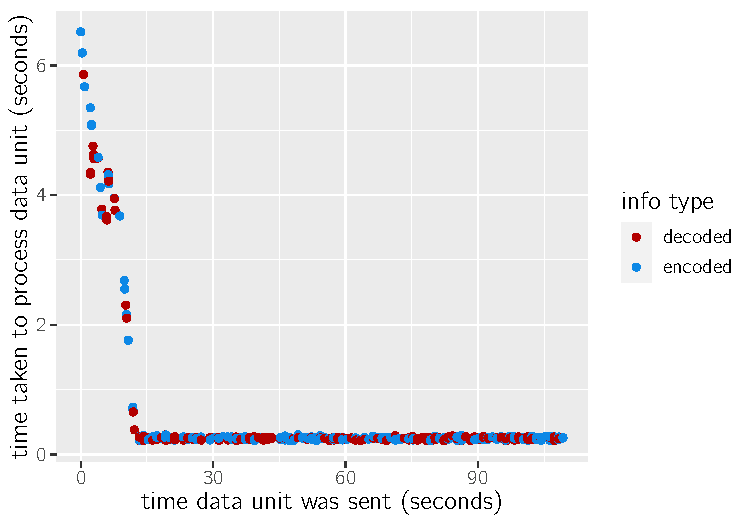
\includegraphics[page=1]{assets/charts/s3eC.pdf}
    \caption[Scatter Chart - Notification Management Scenario - Experience C]{Scatter Chart - Notification Management Scenario - Experience C}
    \label{fig:evaluation:overview:decoproc:chart:s3eC}
\end{figure}

The X axis represents time in seconds since the first request with a data unit was sent, the Y axis represents the time it took for the client to receive the corresponding notification. Each dot represents a data unit.

The data units with the 'decoded' \textit{info type}, in red, were sent to the Data Processor Concern and the ones with the 'encoded' \textit{info type}, in blue, were sent to the Data Decoder Concern.

In conjunction with the chart, the Table~\ref{tab:evaluation:overview:decoproc:results} presents some analysis preformed against the results of Experience C in the Notification Management Scenario.

\begin{table}[H]
    \caption{Metrics collected (in seconds) - Notification Management Scenario - Experience C}
    \label{tab:evaluation:overview:decoproc:results}
    \centering
    \begin{tabular}{@{}ccccccc@{}}
    \toprule
    \textbf{Info Type} & \textbf{Average} & \textbf{Min} & \textbf{Median} & \textbf{Max} & \textbf{90\% Percentile} & \textbf{95\% Percentile} \\ \midrule
    decoded & 0.558 & 0.209 & 0.252 & 5.863 & 0.286 & 3.923 \\ \midrule
    encoded & 0.528 & 0.212 & 0.253 & 6.519 & 0.288 & 3.479 \\ \bottomrule
    \end{tabular}
\end{table}

As we can see the time taken to process or decode a data unit is very similar, this is possible due to \citetitle{graalvm}.

\subsection{Data Flow Caching Process Performance}
\label{subsubsec:evaluation:overview:cache}

The experiences preformed clearly display the process mentioned during the \nameref{chap:design} Chapter in Figure~\ref{fig:design:architecture:platform:container:process:diagram:decoder:2}, about how the \textbf{Data Flow} state is maintained.

In the following charts, Chart~\ref{fig:evaluation:overview:cache:chart:s2eB} and \ref{fig:evaluation:overview:cache:chart:s1eD}, it's possible to envision the various caches in the \textbf{Data Flow} being filled during the first iteration.

\begin{figure}[H]
    \centering
    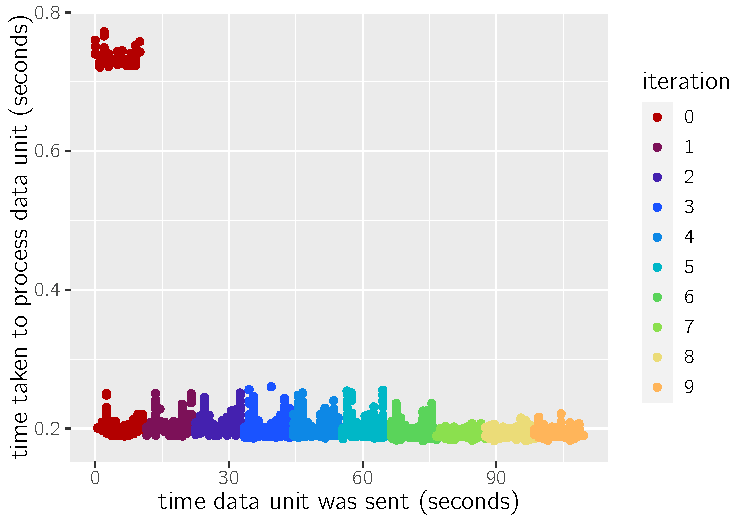
\includegraphics[page=1]{assets/charts/s2eB.pdf}
    \caption[Scatter Chart - Smart Irrigation Scenario - Experience B]{Scatter Chart - Smart Irrigation Scenario - Experience B}
    \label{fig:evaluation:overview:cache:chart:s2eB}
 \end{figure}

\begin{figure}[H]
    \centering
    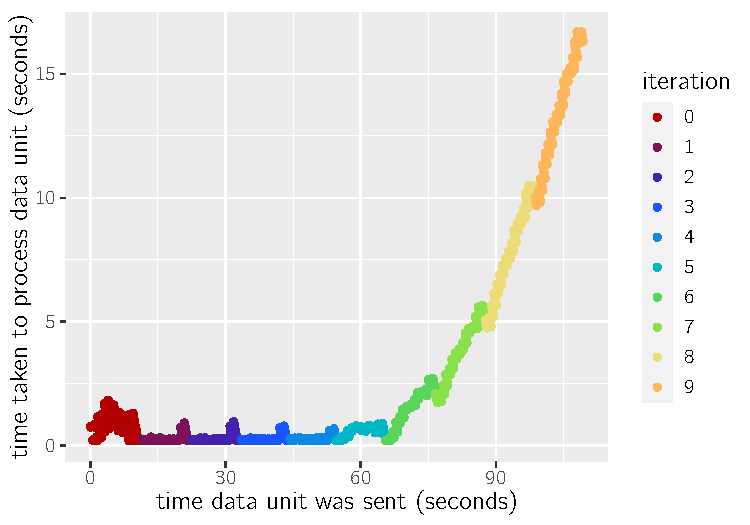
\includegraphics[page=1]{assets/charts/s1eD.pdf}
    \caption[Scatter Chart - Fleet Management Scenario - Experience D]{Scatter Chart - Fleet Management Scenario - Experience D}
    \label{fig:evaluation:overview:cache:chart:s1eD}
\end{figure}

In both charts the X axis represents time in seconds since the first request with a data unit was sent, the Y axis represents the time it took for the client to receive the corresponding measure. Each dot represents a data unit.
Each color represents the test iteration responsible for sending the data unit.

The Chart~\ref{fig:evaluation:overview:cache:chart:s1eD} also that the system started to underperform around the 65 seconds mark. The \textbf{Data Flow} caches were already stable and therefore, under this experiences, it is plausible to say that this process doesn't cause the performance degradation seen in higher throughput experiences.

\subsection{External Services Database Performance}
\label{subsec:evaluation:overview:servicedatabase}

Another important question is wether the performance degradation recorded is due to database access or not.

The experiences performed were able to determine that this was in fact the case with the \textbf{Notification Management Database}, and, to an extent the \textbf{Smart Irrigation Business Database}. As explained in Section~\ref{subsec:implementation:decisions:database},the database used for this containers is \citetitle{postgressql}.
This database, contrary to the one used in \textbf{Fleet Management Data Database} and \textbf{Smart Irrigation Data Database}, is not focused on High-throughput ingestion.

The following chart, Figure~\ref{fig:evaluation:overview:servicedatabase:chart:s4}, shows the discrepancy between storing and serving GPS locations with the \textbf{Fleet Management Backend}. The experiment was performed by mimicking 1500 devices, each sending 10 data units with an interval of around 10 seconds.

This chart represents the number of data units/measures ingested, stored and supplied (Y axis) over time (X axis).

\begin{figure}[H]
    \centering
    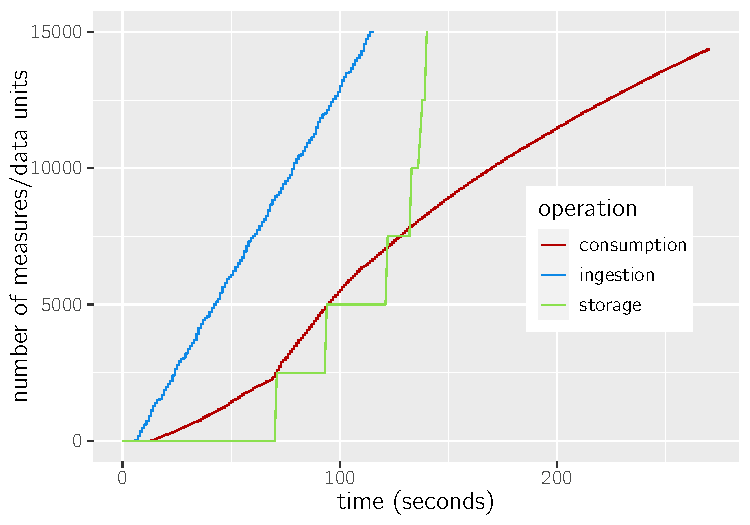
\includegraphics[page=1]{assets/charts/s4.pdf}
    \caption[Line Chart - Time Taken to Ingest, Store and Supply Measures]{Line Chart - Time Taken to Ingest, Store and Supply Measures}
    \label{fig:evaluation:overview:servicedatabase:chart:s4}
\end{figure}

This Chart displays three distinct lines:

\begin{itemize}
    \item Consumption (in red): Measures received by a websocket client connected to the \textbf{Fleet Management Backend};
    \item Ingestion (in blue): Data Units ingested by the \textbf{Data Relayer};
    \item Storage (in green): Measures stored in the \textbf{Fleet Management Data Database}.
\end{itemize}

The data is stored in \citetitle{questdb} via \gls{ILP} and therefore is only committed after a while. The time taken for data to be committed is derived from various parameters and conditions as explained in the Commit Strategy Page\footnote{\href {https://questdb.io/docs/reference/api/ilp/tcp-receiver/\#commit-strategy}{link to QuestDB Commit Strategy Page}} of \citetitle{questdb}.

The chart shows that data is stored long before it is consumed by the websocket client. It also shows that the time between storage and ingestion is relatively small, and once the \textbf{Data Flow} caches stabilize this gap starts to decrease. Implying that the \textbf{Message Broker} does not fall behind the ingestion throughput enforced by the test (136 request per second).

\subsection{System Bottlenecks}
\label{sec:evaluation:overview:bottlenecks}

This section briefly discusses the bottlenecks discovered during the performance tests and analysis preformed.

The components that degraded the test results the most were the GraphQL Subscriptions as envisioned in Figure~\ref{fig:evaluation:overview:servicedatabase:chart:s4}.

The next bottleneck of the solution appears to be the \citetitle{postgressql} Databases, this assessment is based on the result's discrepancy between the three Scenarios.

The experiences \textbf{H} of each scenario, and specially the one related to the platform, foresee that the \textbf{Message Broker} is the next logical bottleneck of the system.

The \nameref{subsec:implementation:description:ingestion} only becomes a bottleneck with a ridiculous amount of devices for a small/medium organization.

If the \textbf{Data Flow} cache sizes are configured correctly, the process of filling them will hardly become a bottleneck, specially since it will be very rare to receive a high number of data units from new devices, decoders or processors that are not already cached.

\section{Synopsis}
\label{sec:evaluation:synopsis}

This evaluation determined that, for the requirements defined in Section~\ref{subsec:requirements:non_functional:performance}, a type \textit{'e2-standard-4'} \gls{VM} instance in Google Cloud Platform was sufficient. The conducted analysis also helped to identify the most important bottlenecks to tackle in the future: (i) GraphQL Subscriptions, (ii) \citetitle{postgressql} Databases, (iii) Message Broker.

The performance tests helped the company to understand the platform limits and how far the production environments are from reaching this limits.

Based on this evaluation, the work described before and the knowledge gathered during the project, the following chapter describes the author opinion regarding the solution.
